% !TeX root = main.tex
\documentclass[a4paper,10pt]{article}
\usepackage{refs/trymtex}
\usepackage{csquotes}
\usepackage[backend=biber]{biblatex}
\usetikzlibrary{matrix}
\usetikzlibrary{positioning,arrows,shapes,calc}

\addbibresource{refs/references.bib}

\title{Numerical Solution of Differential Equations - Project 1}
\author[1]{Sæther, Trym}
\author[1]{Haugen, Tor Ludvig Løvold}
\affil[1]{Department of Mathematical Sciences, NTNU}
\date{\today}

\begin{document}

\maketitle

\tableofcontents
\newpage

\begin{abstract}
\end{abstract}

\section{Problem Description}

In this project, we will study reaction-diffusion equations. Such equations are given by
\begin{equation}
  u_t = \mu u_{xx} + f(u),
\end{equation}

where $\mu$ is some positive constant.
We will assume the reaction term $f(u)$ to be nonstiff, in the sense that explicit methods can be used to solve the ODE $u_t = f(u)$. As is well known, time-dependent PDEs with diffusion terms should be solved by implicit methods. Using implicit methods for solving the whole system requires solutions of nonlinear equations for each step, and we would all be happy to avoid that. One option would be to use an implicit method for the diffusion term and an explicit for the reaction.

We will use constant step sizes $h$ in the $x$-direction, and $k$ in the $t$-direction, so that $x_{m+1} = x_m + h$ and $t_{n+1} = t_n + k$. A scheme based on forward and backward Euler, together with a central difference in space could be
\begin{equation}
  \frac{1}{k} \nabla_t U_m^{n+1}  = \frac{\mu}{h^2} \delta_x^2 U_m^{n+1} + f(U_m^n)
\end{equation}
Which written out could be:
\begin{equation}
  U_m^{n+1}  = U_m^n + r \left( U_{m+1}^{n+1} - 2 U_m^{n+1} + U_{m-1}^{n+1} \right) + k f(U_m^n), \quad r = \frac{\mu k}{h^2}
\end{equation}

We now propose the following modification of the Crank-Nicolson scheme:
\begin{align*}
  U_m^*     & = U_m^n + r \left( \frac{1}{2} \delta_x^2 U_m^* + \frac{1}{2} \delta_x^2 U_m^n \right) + k f(U_m^n) \\
  U_m^{n+1} & = U_m^* + \frac{k}{2} \left( f(U_m^*) - f(U_m^n) \right).
\end{align*}

For pure diffusion ($f = 0$), this is nothing but the usual Crank-Nicolson scheme, and for a pure reaction equation ($\mu = 0$), it is nothing but a second-order explicit Runge-Kutta method.

\begin{railingbox}{Theory problem}
  Do a consistency/stability analysis of the proposed method (1) on a linear PDE, that is, let \(f(u) = au\) for some constant \(a\).
  For the stability analysis, you can choose whether you do a complete matrix analysis for the PDE on a given domain (e.g. \(x \in (0, 1)\)) with boundary conditions, or a Neumann analysis. Is the method unconditionally stable? What can be said about the global error?
  Formulate your results as a mathematical statements (lemmas or theorems) with proofs.
  Justify your theoretical results by numerical experiments.
\end{railingbox}


\begin{railingbox}{Application problem}
  In this exercise, we will look at a model from epidemiology; how an infectious disease will develop in space and time.
  At a given time \(t\), a population \(N\) can be divided into
  \begin{itemize}
    \item Susceptible \(S\): A person is susceptible if she/he may get the disease.
    \item Infective and infectious \(I\): A person is infective if she/he has the disease and is able to transfer it to others.
    \item Removed: \(R\) Part of the population that for some reason will never again be infected or infect others (immune, isolated from the population or dead).
  \end{itemize}
  The following model (SIR) is described in \cite{murray2002mathematical}, chapter 3, and describe the development of a disease over time:
  \begin{align}
    \frac{dS}{dt} & = -\beta SI, \quad \frac{dI}{dt} = \beta SI - \gamma I, \quad \frac{dR}{dt} = \gamma I  \label{eq:sir_model}
  \end{align}
  Notice that \(N(t) = S(t) + I(t) + R(t)\) is constant.
  In the following, we will assume a scaled model, so \(S\), \(I\) and \(R\) are the fraction of the population that are susceptible, infected and removed respectively. In this case, \(S(t) + I(t) + R(t) = 1\).
  The usual SIR model only describe how a disease may develop over time at one specific location, not how a disease is spread in space. Murray \cite{murray2002mathematical}, chapter 13, proposes the following modification to include spatial spread:
  \begin{align}
    S_t & = -\beta IS + \mu S \Delta S, \nonumber                            \\
    I_t & = \beta IS - \gamma I + \mu I \Delta I, \label{eq:sir_model_space}
  \end{align}
  where \(\Delta u = u_{xx} + u_{yy}\) (see the appendix). Your exercise is now: Try to understand the
  model. Choose an appropriate numerical scheme for solving the PDEs, and use this to study the spread of a disease. That is, at \(t = 0\) assume a small portion of the population is infected at some particular place, and see how the disease
  will spread from there. You are free to choose the domain, the parameters and boundary conditions, but you should be able to get some interesting results out of it. And you should justify your choices.
  As soon as you have a working model, play with it! As an example: In the present model, we assume that the population is equally distributed over the domain. You can for instance model a more dense populated area (or an event that gather a lot of people) by making \(\beta\) larger over there (and then dependent on \(x\)).
  Some hints:
  \begin{itemize}
    \item To get a certain feeling for the dynamics of the model, solve \eqref{eq:sir_model} first. As a first try, you can use \(\beta = 3\) and \(\gamma = 1\), but then change the parameters and see what happens. Use a standard ODE solver if you prefer.
    \item The diffusion parameters \(\mu^*\) describes how fast people are moving around. If your domain is small, you should probably use quite small diffusion parameters.
    \item For a full score, the 2d problem should be solved. But if this seems difficult, solve the 1d problem first.
  \end{itemize}
\end{railingbox}





\chapter{Introduction}
\section{Theory}

\subsection{Theoretical Background}

\begin{definition}{Local Truncation Error}{lte}
  The local truncation error (LTE) is the error made at a single grid point when approximating a differential equation with a finite difference scheme.
  \[
    \norm{\tau_m^n} = \norm{u(x_m, t_n) - U_m^n} = \mathcal{O}(h^p + k^q) \quad \text{as} \quad h, k \to 0
  \]
  where \(p\) and \(q\) are the order of the spatial and temporal discretizations, respectively.
\end{definition}


\paragraph{Taylor Expansions}

\subparagraph{Spatial Taylor Expansions}
\begin{align*}
  u_{m+1}^n & \approx u_m^n + h \partial_x u_m^n + \frac{h^2}{2} \partial_x^2 u_m^n + \frac{h^3}{6} \partial_x^3 u_m^n + \mathcal{O}(h^4) \\
  u_{m-1}^n & \approx u_m^n - h \partial_x u_m^n + \frac{h^2}{2} \partial_x^2 u_m^n - \frac{h^3}{6} \partial_x^3 u_m^n + \mathcal{O}(h^4) \\
\end{align*}

\subparagraph{Temporal Taylor Expansions}
\begin{align*}
  u_m^{n+1} & \approx u_m^n + k \partial_t u_m^n + \frac{k^2}{2} \partial_t^2 u_m^n + \frac{k^3}{6} \partial_t^3 u_m^n + \mathcal{O}(k^4)                                                                                                            \\
  u_m^\star & \approx u_m^n + \Phi k \partial_t u_m^n + \frac{(\Phi k)^2}{2} \partial_t^2 u_m^n + \frac{(\Phi k)^3}{6} \partial_t^3 u_m^n + \mathcal{O}(k^4)                                                                                         \\
            & = u_m^n + \Phi k \left(\mu \partial_x^2 u_m^n + a u_m^n\right) + \frac{(\Phi k)^2}{2} \left(\mu \partial_x^2 \left(\mu \partial_x^2 u_m^n + a u_m^n\right) + a \left(\mu \partial_x^2 u_m^n + a u_m^n\right)\right) + \mathcal{O}(k^4) \\
\end{align*}

\subparagraph{Spatial and Temporal Taylor Expansion}
\begin{align*}
  u_{m+1}^\star & \approx u_m^n + \left(\Phi k \partial_t u_m^n + h \partial_x u_m^n\right) + \frac{1}{2}\left(\Phi^2 k^2 \partial_t^2 u_m^n + h^2 \partial_x^2 u_m^n\right) + \mathcal{O}(h^3 + k^3) \\
  u_{m-1}^\star & \approx u_m^n + \left(\Phi k \partial_t u_m^n - h \partial_x u_m^n\right) + \frac{1}{2}\left(\Phi^2 k^2 \partial_t^2 u_m^n + h^2 \partial_x^2 u_m^n\right) + \mathcal{O}(h^3 + k^3) \\
\end{align*}
\subparagraph{Operator Taylor Expansion}
\begin{align*}
  \delta_x^2 u_m^n = u_{m+1}^n - 2u_m^n + u_{m-1}^n = h^2\partial_{xx}u_m^n + \mathcal{O}(h^4) \\
  \delta_x^2 u_m^\star = u_{m+1}^\star - 2u_m^\star + u_{m-1}^\star = h^2\partial_{xx}u_m^n + \mathcal{O}(h^4 + k^4) \\
\end{align*}

\paragraph{Notation}
\begin{tabular}{ll}
  \textbf{Symbol}               & \textbf{Meaning}                       \\
  \hline                                                                 \\[-1em]
  \(u = u(x, t)\)               & Exact temperature distribution         \\
  \(u_m^n = u(x_m, t_n)\)       & Exact temperature at grid point        \\
  \(\mu\)                       & Diffusion coefficient                  \\
  \(f(u)\)                      & Reaction term                          \\
  \(u_0(x)\)                    & Initial temperature distribution       \\
  \(g(x, t)\)                   & Boundary condition                     \\
  \(\Omega\)                    & Spatial domain                         \\
  \(\partial \Omega\)           & Boundary of spatial domain             \\
  \hline                                                                 \\[-1em]
  \(U_m^n \approx u(x_m, t_n)\) & Numerical approximation of temperature \\
  \(x_m = m h\)                 & Spatial grid points                    \\
  \(t_n = n k\)                 & Temporal grid points                   \\
  \(h = L/M\)                   & Spatial step size                      \\
  \(k =T/N\)                    & Temporal step size                     \\
  \(L\)                         & Spatial domain length                  \\
  \(T\)                         & Final time                             \\
  \(M\)                         & Number of spatial grid points          \\
  \(N\)                         & Number of temporal grid points         \\
  \(\mathbb{G}\)                & Set of all grid points                 \\
  \hline
\end{tabular}


\subsection{The Heat Equation}

The heat equation is a fundamental partial differential equation (PDE) that governs how temperature evolves in a given region over time. In its simplest form, we consider a one-dimensional case in which heat flows along a single spatial dimension:
\begin{align*}
  \frac{\partial u}{\partial t} & = \mu \frac{\partial^2 u}{\partial x^2} + f(u), \quad \left( x, t \right) \in \Omega \times \left(0, T\right) \tag{PDE} \\
                                &
  \begin{cases}
    u(x, 0) = u_0(x)  &                       \\
    u(0, t) = g(x, t) & x \in \partial \Omega \\
  \end{cases} \tag{BC}
\end{align*}\label{eq:heat_eq}

The equation describes how the temperature \(u(x, t)\) at position \(x\) and time \(t\) evolves over time.

\paragraph{Diffusion and Reaction Terms}
The diffusion term \(\mu \frac{\partial^2 u}{\partial x^2}\) describes how heat spreads through the material, while the reaction term \(f(u)\) accounts for any heat sources or sinks in the system.

\paragraph{Initial and Boundary Conditions}
The initial temperature distribution \(u_0(x)\) and boundary condition \(g(x, t)\) specify the temperature at the start and where heat enters or leaves the system, respectively.

\paragraph{Parabolic PDE}
The heat equation is a \emph{parabolic} PDE describing how processes evolve over time. For numerical solutions, the spatial and temporal domains are discretized, and the solution is approximated at discrete points. Finite difference methods efficiently handle these discretizations, allowing accurate approximations of the evolving temperature.

\subsubsection{Discretization of the Heat Equation}
Discretizing the heat equation involves dividing the spatial domain \(\Omega\) into \(M\) equally spaced points, with \emph{step length \(h\)} and the temporal domain into \(N\) steps, with \emph{step size \(k\)}.
Each grid point is denoted by \((x_m, t_n)\), where \(x_m = m h\) and \(t_n = n k\) for \(m = 0, \ldots, M\) and \(n = 0, \ldots, N\). The solution \(U_m^n\) approximates the temperature \(u(x_m, t_n)\) at each grid point.

\begin{minipage}[l]{0.45\textwidth}
  \begin{align*}
    U_m^n      & \approx u(x_m, t_n) \quad \text{for } (x_m, t_n) \in \mathbb{G} \\[1em]
    \mathbb{G} & := \left\{(x_m, t_n):
    \begin{cases}
      x_m = m h & h = L/M, m = 0, \ldots, M \\
      t_n = n k & k = T/N, n = 0, \ldots, N
    \end{cases}\right\}
  \end{align*}\label{eq:grid_points}
  Where \(L\) is the spatial domain length and \(T\) is the final time.
  \begin{remark}{Constant Grid Spacing}{step_sizes}
    For simplicity, \(h\) and \(k\) are constant \( x_{m+1} = x_m + h,\quad t_{n+1} = t_n + k \).
  \end{remark}

\end{minipage}
\hspace{0.05\textwidth}
\begin{minipage}[r]{0.45\textwidth}
  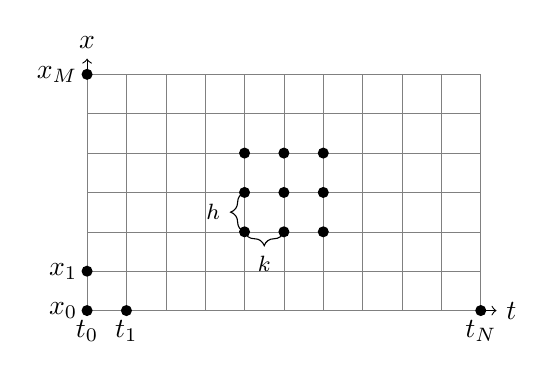
\begin{tikzpicture}
    % Axes
    \draw[->] (0,0) -- (5.2,0) node[right] {\(t\)};
    \draw[->] (0,0) -- (0,3.2) node[above] {\(x\)};

    % Grid points
    \draw[step=0.5cm,gray,very thin] (0,0) grid (5,3);

    \node[below] at (0,0) {\(t_0\)};
    \node[below] at (0.5,0) {\(t_1\)};
    \node[below] at (5,0) {\(t_N\)};
    \node[left] at (0,0) {\(x_0\)};
    \node[left] at (0,0.5) {\(x_1\)};
    \node[left] at (0,3) {\(x_M\)};

    % Add some key points with labels
    \foreach \x in {2,2.5,3} {
        \foreach \y in {1,1.5,2} {
            \fill (\x,\y) circle (2pt);
          }
      }

    % Add curly braces to show length k and h on axes
    \draw [decorate,decoration={brace,amplitude=5pt}]
    (2.5,1) -- (2,1) node [black,midway,yshift=-0.4cm] {\footnotesize \(k\)};
    \draw [decorate,decoration={brace,amplitude=5pt}]
    (2,1) -- (2,1.5) node [black,midway,xshift=-0.4cm] {\footnotesize \(h\)};

    % Add circles/points at nodes
    \fill (0,0) circle (2pt);
    \fill (0.5,0) circle (2pt);
    \fill (5,0) circle (2pt);
    \fill (0,0.5) circle (2pt);
    \fill (0,3) circle (2pt);
  \end{tikzpicture}
\end{minipage}

\subsection{Finite Difference Schemes}
Finite difference methods approximate differential equations by replacing them with a system of algebraic equations on the chosen grid.
The heat equation is often solved with these methods for their simplicity and computational efficiency.

\paragraph{The Forward-Time Central-Space (FTCS) scheme}
FTSC is a simple and widely used method for solving the heat equation.
It approximates the time derivative with a forward difference and the spatial derivative with a central difference.

\begin{align*}
  \frac{1}{k} \nabla_t U_m^{n+1} & = \frac{\mu}{h^2} \delta_x^2 U_m^{n+1} + f(U_m^n)                                              \\
  \nabla_t U_m^{n+1}             & = r \delta_x^2 U_m^{n+1} + k f(U_m^n), \quad r = \frac{\mu k}{h^2}                             \\
  U_m^{n+1}                      & = U_m^n + r \left( U_{m+1}^{n+1} - 2 U_m^{n+1} + U_{m-1}^{n+1} \right) + k f(U_m^n) \tag{FTCS}
\end{align*}

\paragraph{Crank-Nicolson Scheme}

The Crank-Nicolson scheme is an implicit method that approximates the spatial derivative at the midpoint between time steps. It is unconditionally stable and second-order accurate in time and space.
\begin{align*}
  U_m^\star & = U_m^n + \frac{r}{2} \left( \delta_x^2 U_m^\star + \delta_x^2 U_m^n \right) + k f(U_m^n), \quad r = \frac{\mu k}{h^2} \tag{Crank-Nicolson} \\
  U_m^{n+1} & = U_m^\star + \frac{k}{2} \left( f(U_m^\star) - f(U_m^n) \right)
\end{align*}

\subsection{Error Analysis}
Given the function \(f(u) = au\) for constant \(a\), we first want to analyze the consistency of the Crank-Nicolson scheme by determining the local truncation error (LTE).

\subsubsection{Consistency analysis (Local Truncation Error)}
The local truncation error (LTE) is the error at a single grid point when approximating a differential equation with a finite difference scheme.
It is the difference between the exact solution \(u(x_m, t_n)\) and the numerical approximation \(U_m^n\).

\begin{theorem}{Local truncation error for Crank-Nicolson}{lte_cn}
  Consider the heat equation with linear reaction term \(f(u) = au\) for constant \(a\), discretized using the Crank-Nicolson scheme. Let \(u_m^n = u(x_m,t_n)\) denote the exact solution at grid points and \(u_m^\star = u(x_m, t_n + \Phi k)\) for \(\Phi \in [0,1]\) be an intermediate solution.

  The local truncation error \(\tau_m^n = \norm{u(x_m, t_n) - U_m^n}\) satisfies
  \[
    \norm{\tau_m^n} = \mathcal{O}(k + \tfrac{h^4}{k})
  \]
  When choosing the time step \(k \sim h^2\), the scheme achieves second-order accuracy in both time and space:
  \[
    \norm{\tau_m^n} = \mathcal{O}(h^2 + k^2)
  \]
\end{theorem}
\begin{proof}[Proof of Theorem~\ref{thm:lte_cn}]

  We will use Taylor expansions around $(x_m, t_n)$ in both space and time~\ref{eq:taylor}.

  From central differences, we have
  \[
    \delta_x^2 u_m^n = h^2\partial_{xx}u_m^n + \mathcal{O}(h^4)
  \]
  Since $u_m^\star = u(x_m, t_n+\Phi k)$, similar Taylor expansions yield
  \[
    \delta_x^2 u_m^\star
    = u_{m+1}^\star - 2u_m^\star + u_{m-1}^\star
    = h^2\partial_{xx}u_m^n + \mathcal{O}\bigl(h^4 + k^4\bigr).
  \]

  Substitute these into the Crank--Nicolson half-step:
  \[
    U_m^\star
    = U_m^n
    + \frac{r}{2}\bigl(\delta_x^2 U_m^\star + \delta_x^2 U_m^n\bigr)
    + kaU_m^n,
    \quad
    r = \frac{\mu k}{h^2}.
  \]
  Matching $U_m^\star$ with the exact solution plus higher-order terms, we get
  \[
    U_m^\star
    = u_m^n
    + rh^2\partial_{xx}u_m^n
    + kau_m^n
    + \mathcal{O}\bigl(h^4 + k^4\bigr).
  \]

  Next, we compute the full step using the intermediate solution:

  \[
    U_m^{n+1}
    = U_m^\star
    + \tfrac{k}{2}\bigl(aU_m^\star - aU_m^n\bigr).
  \]
  Expand $U_m^\star$ in time around $(x_m,t_n)$ and collect terms carefully:
  \[
    U_m^{n+1}
    = u_m^n
    + k\partial_t u_m^n
    + \tfrac{k^2}{2}\partial_t^2 u_m^n
    + \tfrac{k^3}{6}\partial_t^3 u_m^n
    + \tfrac{ark}{2}h^2\partial_{xx} u_m^n
    + \tfrac{a^2k^2}{2}u_m^n
    + \mathcal{O}\bigl(k^4 + h^4\bigr).
  \]

  Since $rh^2 = \mu k$, the term involving $\partial_{xx} u_m^n$ can be written as
  $\tfrac{a\mu k^2}{2}\partial_{xx}u_m^n$.

  Compare to the exact solution at the next time level:

  \[
    u_m^{n+1}
    = u_m^n
    + k\partial_t u_m^n
    + \tfrac{k^2}{2}\partial_t^2 u_m^n
    + \tfrac{k^3}{6}\partial_t^3 u_m^n
    + \mathcal{O}\bigl(k^4\bigr).
  \]

  Their difference is
  \[
    U_m^{n+1} - u_m^{n+1} =
    \underbrace{\left(\tfrac{a\mu k^2}{2}\partial_{xx}u_m^n
      + \tfrac{a^2k^2}{2}u_m^n\right)}_{\mathcal{O}(k^2)}
    + \mathcal{O}\left(k^3 + h^4\right)
    = \mathcal{O}\left(k^2 + h^4\right).
  \]
  Thus, the local truncation error (per time step) is
  \[
    \lVert{\tau_m^n}\rVert
    = \left\lVert\dfrac{1}{k}\left(U_m^{n+1} - u_m^{n+1}\right) \right\rVert
    = \mathcal{O}\bigl(k + \tfrac{h^4}{k}\bigr).
  \]
  If we choose $k \sim h^2$, then
  \[
    \frac{h^4}{k} \sim h^2,
    \quad
    \Rightarrow
    \quad
    \lVert{\tau_m^n}\rVert \approx \mathcal{O}\bigl(k^2 + h^2\bigr).
  \]
  Therefore, under the usual choice $k \propto h^2$, the scheme is second-order accurate in both time and space. \qed
\end{proof}

\subsubsection{Stability Analysis (Von Neumann Stability)}
The Von Neumann stability analysis is a method to determine the stability of a finite difference scheme by analyzing the growth of errors in the Fourier modes of the solution.
\begin{theorem}{Stability of the Crank-Nicolson scheme}{stability_cn}
  The Crank-Nicolson scheme is stable for the heat equation with linear reaction term \(f(u) = au\) if:
  \[
    ka \leq 0.618 \quad \text{and} \quad \frac{\mu k}{h^2}(\cos\beta - 1) \leq 0
  \]
  Under these conditions, the amplification factor satisfies \(\norm{\xi} \leq 1\).
\end{theorem}
\begin{proof}[Proof of Theorem~\ref{thm:stability_cn}]
  Let \(U_m^n = \xi^n e^{i m \beta}\) be the Fourier mode of the numerical solution at grid point \((x_m, t_n)\), where \(\xi=\dfrac{\xi^{n+1}}{\xi^n}\) is the amplification factor and \(\beta\) is the wave number.
  For the first step of the Crank-Nicolson scheme, we have:
  \begin{align*}
    U_m^\star               & = U_m^n + \dfrac{r}{2} (\delta_x^2 U_m^\star + \delta_x^2 U_m^n) + k a U_m^n                                                                     \\
    \xi^\star e^{i m \beta} & = \xi^n e^{i m \beta} + \dfrac{r}{2} \left(\xi^\star + \xi^n\right)\left(e^{i\beta} - 2 + e^{-i\beta}\right)e^{im\beta}+ k a \xi^n e^{i m \beta} \\
    \xi^\star               & = \xi^n + \dfrac{r}{2} \left(\xi^\star + \xi^n \right)\overbrace{\left(e^{i \beta} - 2 + e^{-i \beta}\right)}^{2\cos\beta - 2} + k a \xi^n       \\
    \xi^\star               & = (1 + r(\cos\beta - 1) + ka) \xi^n + r(\cos\beta - 1)\xi^\star                                                                                  \\
    \xi^\star               & = \dfrac{1 + \alpha + \sigma}{1 - \sigma} \xi^n \quad \text{where } \alpha = ka, \sigma = r(\cos\beta - 1)
  \end{align*}
  Then, for the second step, we get:
  \begin{align*}
    U_m^{n+1}               & = U_m^\star + \tfrac{\alpha}{2}(U_m^\star - U_m^n)                                                                      \\
    \xi^{n+1} e^{i m \beta} & = \xi^\star e^{i m \beta} + \tfrac{\alpha}{2}(\xi^\star - \xi^n)e^{i m \beta}                                           \\
    \xi^{n+1}               & = (1 + \tfrac{\alpha}{2}) \xi^\star - \tfrac{\alpha}{2} \xi^n                                                           \\
    \xi^{n+1}               & = \left(1 + \tfrac{\alpha}{2}\right)\left(\tfrac{1 + \alpha + \sigma}{1 - \sigma}\right)\xi^n - \tfrac{\alpha}{2} \xi^n \\
    \xi                     & = \tfrac{\xi^{n+1}}{\xi^n} = -\dfrac{\alpha^2 + 2(\alpha + 1) (\sigma + 1)}{2 (\sigma - 1)} \tag{Source: Trust me bro}
  \end{align*}
  Furthermore, we can now find a bound for the amplification factor:
  \begin{align*}
    \norm*{\xi}                                    & = \norm*{-\dfrac{\alpha^2 + 2(\alpha + 1)(\sigma + 1)}{2(\sigma - 1)}} \leq \dfrac{\alpha^2}{2\underbrace{\abs*{\sigma - 1}}_{\geq 1}} + \dfrac{(\alpha + 1)\overbrace{\abs*{\sigma + 1}}^{\leq 1}}{2\underbrace{\abs{\sigma - 1}}_{\geq 1}} \leq \dfrac{\alpha^2+ \alpha + 1}{2} \leq 1 \\                                                                                                                                                                                                                     \\
    \tfrac{1}{2}\left(\alpha^2 + \alpha - 1\right) & \leq 0 \Rightarrow \alpha_{1,2} = \tfrac{1}{2}\left(-1 \pm \sqrt{5}\right) \approx -1.618, 0.618 \Rightarrow \alpha \leq 0.618                                                                                                                                                           \\
    \norm*{\xi}                                    & \leq 1 \implies \alpha \leq 0.618 \text{ and } \sigma = \frac{\mu k}{h^2}(\cos\beta - 1) \leq 0 \tag{Stability}
  \end{align*}
\end{proof}

\paragraph{\color{red} Is the method unconditionally stable?}

\paragraph{\color{red} What can be said about the global error?}

\begin{align*}
  \mathcal{L}_h U_m^{n+1} & = U_m^\star + \tfrac{ka}{2} \left( U_m^\star - U_m^n \right)                                                                                                                                 \\
                          & = \left(U_m^n + \frac{r}{2} \left( \delta_x^2 U_m^{n+\phi} + \delta_x^2 U_m^n \right) + k a U_m^n\right) + \tfrac{ka}{2} \left( U_m^{n+\phi} - U_m^n \right)                                 \\
                          & = u_m^n + k\partial_t u_m^n + \tfrac{k^2}{2}\partial_t^2 u_m^n + \tfrac{k^3}{6}\partial_t^3 u_m^n + \tfrac{ark}{2}h^2\partial_{xx} u_m^n + \tfrac{a^2k^2}{2}u_m^n + \mathcal{O}(k^4+h^4)
\end{align*}

\subsection{\color{red} Numerical Experiments}
\section{Application}

\subsection{SIR Model}
\begin{align}
  \begin{cases}
    S_t & = -\beta IS + \mu_S \Delta S           \\
    I_t & = \beta IS - \gamma I + \mu_I \Delta I
  \end{cases}
  \implies
  \begin{cases}
    \frac{\partial S}{\partial t} & = -\beta IS + \mu_S\left(\frac{\partial^2 }{\partial x^2}S + \frac{\partial^2 }{\partial y^2} S \right)            \\
    \frac{\partial I}{\partial t} & = \beta IS - \gamma I + \mu_I \left(\frac{\partial^2 }{\partial x^2}I  + \frac{\partial^2 }{\partial y^2} I\right)
  \end{cases}
\end{align}

\subsubsection{Discretization}

\begin{align*}
  u_{i,j}^n & = u(x_i,y_j,t_n) \tag{exact}                                                       \\
  U_m^n     & \approx u(x_m,y_j,t_n) \tag{approx}                                                \\
  x_i       & = ih = i\frac{1}{M}, \quad y_j = j = j\frac{1}{M} & \text{for } i,j = 0,1,\ldots,M \\
  t_n       & = nk = n\frac{1}{N}                               & \text{for } n = 0,1,\ldots,N
\end{align*}

\subsubsection{Method}
\begin{align*}
  \partial_x^2 U_{i,j}^n & = \frac{1}{h^2} \left(U_{i+1,j}^n - 2U_{i,j}^n + U_{i-1,j}^n \right) + \mathcal{O}(h^2)                                                                   \\
  \partial_y^2 U_{i,j}^n & = \frac{1}{h^2} \left(U_{i,j+1}^n - 2U_{i,j}^n + U_{i,j-1}^n\right) + \mathcal{O}(h^2)                                                                    \\
  \partial_t U_{i,j}^n   & = \frac{1}{k^2} \left(U_{i+1,j}^n + U_{i-1,j}^n + U_{i,j+1}^n + U_{i,j-1}^n - 4U_{i,j}^n\right) + \mathcal{O}(k^2) \quad \text{for } i,j = 1,2,\ldots,M-1
\end{align*}

\subsubsection{Scheme}

\paragraph{Susceptible}

\begin{align*}
  \partial_t S                                        & = -\beta IS + \mu_S \left(\partial_x^2 S + \partial_y^2 S\right)                                                                                                                                                                       \\
  \frac{1}{h}\left(S_{i, j}^{n+1} - S_{i, j}^n\right) & =  - \beta \mathcal{I}_{i,j}^n \mathcal{S}_{i,j}^n +  \frac{\mu_S}{h^2} \left(\mathcal{S}_{i+1,j}^n + \mathcal{S}_{i-1,j}^n + \mathcal{S}_{i,j+1}^n + \mathcal{S}_{i,j-1}^n - 4\mathcal{S}_{i,j}^n\right) + \mathcal{O}(h^2)           \\
  S_{i,j}^{n+1}                                       & = h \left(1 - \beta\mathcal{I}_{i,j}^n - \dfrac{4\mu_S}{h^2}\right)\mathcal{S}_{i,j}^n + \frac{\mu_S}{h} \left(\mathcal{S}_{i+1,j}^n + \mathcal{S}_{i-1,j}^n + \mathcal{S}_{i,j+1}^n + \mathcal{S}_{i,j-1}^n\right) + \mathcal{O}(h^2)
\end{align*}



\clearpage
\paragraph{Infected}
\noindent
\begin{align*}
  \partial_t \mathcal{I}                                                & = \beta \mathcal{I}\mathcal{S} - \gamma \mathcal{I} + \mu_I \left(\partial_x^2 + \partial_y^2\right)\mathcal{I}                                                                                                                                      \\
  \frac{1}{h}\left(\mathcal{I}_{i,j}^{n+1} - \mathcal{I}_{i,j}^n\right) & = \beta \mathcal{I}_{i,j}^n \mathcal{S}_{i,j}^n - \gamma \mathcal{I}_{i,j}^n + \frac{\mu_I}{h^2}\left(\mathcal{I}_{i+1,j}^n + \mathcal{I}_{i-1,j}^n + \mathcal{I}_{i,j+1}^n + \mathcal{I}_{i,j-1}^n - 4\mathcal{I}_{i,j}^n\right) + \mathcal{O}(h^2) \\
  \mathcal{I}_{i,j}^{n+1}                                               & = \left(1 + \beta\mathcal{S}_{i,j}^n - \gamma - \dfrac{4\mu_I}{h^2}\right)\mathcal{I}_{i,j}^n + \frac{\mu_I}{h}\left(\mathcal{I}_{i+1,j}^n + \mathcal{I}_{i-1,j}^n + \mathcal{I}_{i,j+1}^n + \mathcal{I}_{i,j-1}^n\right) + \mathcal{O}(h^2)
\end{align*}



\printbibliography

\appendix
\subsection{Appendix: Python Code}
\inputminted{python}{simulation/SIRSimulation.py}
\inputminted{python}{simulation/application.py}

\end{document}
